\chapter{Thermomechanical behavior of semi-crystalline polymers} \label{ch:thermomechanical_behavior_semi_crystalline_polymer}


% order of magnitude difference

% Why polymers good design.
%
%   Employ all props for comparison with metals, ceramics and composites.
%
%   stiff and yield vs densitiy. Polymer best if low weight is benefit.
%
%   Polymer not as though
%
%   Polymers best at strain failure.
%
%   comparison amorphous vs semi-crystalline
%
%    Manufacturing.
%    Thermoplastics dominate the market due to their reduced production costs, energy efficiency, ability to , and ability to be produced in extremely high volumes with high precision and at a cheap cost.
%    They possess a clear melting point where the material transitions to a viscous melt, in contrast to amorphous polymers which soften continously after the glass transition temperature until they reach a similar state.
%

% Nylon 101 is a standard all-purpose extruded grade of nylon type 66 (polyamide). Also, among all of the unmodified nylons, it is the strongest, hardest nylon, and has one of the highest melting temperatures (260 C or 500 F)

% applications of semi-crystalline

% continuous use.

% Polyethylene is a semi-crystalline polymer which can be manufactured with degrees of crystallinity ranging from 15\% to 70\% \citep{ayoubEffectsCrystalContent2011}, e.g., by controlling the amount of branching in the polyethylene macromolecules \citep{schrauwenIntrinsicDeformationBehavior2004}.

% density arround \SI{1}{\killo\gram\per\centi\meter^3}
% young modulus ranging from \SIrange{0.1}{10}{\giga\pascal}
% strength from below \SIrange{10}{100}{\mega\pascal} above.
% Large failure strains max energy storage per unit volume \SIrange{0.01}{0.1}{} 10 times larger than metals
% good combination specific strength and young modulus, better only composite and ceramic compressive , semi-crystalline
% Intrinsic damping
% Low thermal conductivity of the order of \SI{0.1}{\watt\per\meter\per\kelvin} and low diffusivity \SI{10e-7}{\meter^2\per\second}.
% Bad thermal distortion as $\alpha$ \SIrange{3e-5}{4e-4}{\per\kelving} is large 10 metal 100 ceramics
% Relatively low thermal stresses.
% high temperature not incredible
% PTFE the best on friction and uhwpe  ldfpe anylon hovering around 0.1
% goog wear rate PTFE HDPE
% salt water, strong acids, strong alkalis, organic solvents, uv radiation, aerate water.

The goal of this chapter is to clearly outline the thermomechanical response of semi-crysatlline polymers.
An account of their deformation mechanisms opens the chapter, followed by the experimental results of various mechanical experiments, such as constant strain rate, stress relaxation, and creep tests.
An appropriate discussion regarding their dependency on factors such as temperature, the strain rate or the pressure is also included.
Closing the chapter are the results of thermal analysis techniques, such as differential scanning calorimetry.

An effort is made to provide relevant literature references where the experimental results can be found.
Some of them are later used in the validation and comparison of the various models available in the literature.

\section{Deformation mechanisms for semi-crystalline polymers}
A deformation mechanism is a kinetic process occurring at the atomic, microscopic or mesoscopic scale responsible for changes in a material's internal structure, shape or volume, implying a characteristic deformation behavior, i.e., a constitutive relation between stress, strain, strain rate and temperature \citep{frostDeformationmechanismMapsPlasticity1982}.
According to Arzhakov \citep{arzhakovRelaxationPhysicalMechanical2019}  it corresponds, in general, to:
\begin{enumerate}
	\item molecular-kinetic aspects, such as the mutual torsional-vibrational and translational motions of microscopic kinetic units of various sizes;
	\item structural aspects, such as the creation/annihilation of kinetic units or change in the resistance to their motion,
\end{enumerate}
where a kinetic unit is a structural element possessing vibrational and translational degrees of freedom.
As a rule of thumb, the molecular-kinetic aspects by themselves describe a steady state, such that the stress and the temperature determine completely the strain rate, and other variables characterizing the structure of the material.
The structural aspects will lead to a transient beahvior, meaning that the stress and the temperature will not be enough to determine the response of the material, since the structure is also changing \citep{frostDeformationmechanismMapsPlasticity1982}.

One way to study the deformation mechanisms in a polymer is to consider its relaxation transitions.
A relaxation transition is a change in the material's response to an external action caused by the mobility of a specific kinetic unit in a given temperature-time test mode.
No irrecoverable deformation or structure change are allowed, however \citep{arzhakovRelaxationPhysicalMechanical2019}.
The range of experimental approaches and techniques for the study of relaxation phenomena is extremely diverse and includes isochronal--considering the response at the same instant or at the same frequency--and isothermic results from experiments such as thermomechanical analysis, differential scanning calorimetry (DSC) \nomenclature[A]{DSC}{\textbf Differential \textbf Scanning \textbf calorimetry} (reviewed in more detail below), dielectric and acoustic measurements, radio thermoluminescence, nuclear magnetic resonance, various modifications of probe methods, among others \citep{ferryViscoelasticPropertiesPolymers1980, arzhakovRelaxationPhysicalMechanical2019}.

Despite the partially ordered structure of the crystalline phase and the limitation of molecular mobility imposed by it, the relaxation spectra of a semi-crystalline polymer is generally richer than that of a glassy polymer.
The kinetic units in the former can be made to correspond to features inside crystallites, in the intercrystalline amorphous region, or on the surface of the crystallites \citep{ferryViscoelasticPropertiesPolymers1980, arzhakovRelaxationPhysicalMechanical2019}.

The assignment of a given relaxation transition to a deformation mechanism within a phase of the semi-crystalline polymer can be achieved in two ways: (i) considering the same polymer at different degrees of crystallinity, lamellar thicknesses, defect content, cross-linking; \citep{ferryViscoelasticPropertiesPolymers1980}, and (ii) employing an etching procedure \citep{arzhakovRelaxationPhysicalMechanical2019}.
Hoffman et al. \citep{hoffmanAnalysisRelaxationsPolychlorotrifluoroethylene2007}, when discussing the relaxation behavior of polycholorotrifluoroethylene (PCTFE) \nomenclature[A]{PCTFE}{\textbf{P}oly\textbf{c}holoro\textbf{t}ri\textbf{f}luoro\textbf{e}thylene}  and polyethylene (PE)  \nomenclature[A]{PE}{\textbf{P}oly\textbf{e}thylene}, describe deformation mechanisms such as the motion of chain folds coupled with interior chains and relaxation at chain-end induced row vacancies in chain-folded crystals.
The relaxation behavior of semi-crystalline polymers are discussed later with thermomechanical experiments as a basis, both isotermic and isochronal.
Some of the kinetic units responsible for the deformation mechanism in a semi-crystalline polymer are \citep{arzhakovRelaxationPhysicalMechanical2019}:
\begin{enumerate}
	\item between the crystalline cores of the lamellas;
	\item regular folds with suppressed mobility;
	\item irregular loops;
	\item folded tie-chains;
	\item free ends of macromolecules coming out of lamellas;
	\item slightly curved tie-chains;
	\item folds the mobility of which is significantly limited by crystallites;
	\item fully straightened tie-chains, the ends of which are fixed by neighbouring lamellas.
\end{enumerate}
See Figure~\ref{fig:kinetic_units_relax_scp} for their schematic depiction.
\begin{figure}[hbtp]
	\centering
	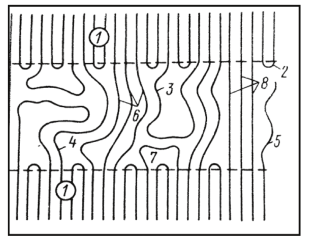
\includegraphics[width=0.6\textwidth]{figures/kinetic_units_scp}
	\caption{Schematic depiction of the kinetic units associated with relaxation transitions in lamellar PE. 1) between the crystalline cores of the lamellas; 2) regular folds with suppressed mobility; 3) irregular loops; 4) folded tie-chains; 5) free ends of macromolecules coming out of lamellas; 6) slightly curved tie-chains; 7) folds the mobility of which is significantly limited by crystallites; 8) fully straightened tie-chains, the ends of which are fixed by neighbouring lamellas. Taken from \cite{arzhakovRelaxationPhysicalMechanical2019}.}
\label{fig:kinetic_units_relax_scp}
\end{figure}

Bowden and Young \citep{bowdenDeformationMechanismsCrystalline1974} provide an early description of the deformation mechanisms in a semi-crystalline polymer not associated with relaxation transitions.
These may include structural changes and lead to permanent deformation.
Drozdov et al. \citep{drozdovViscoelasticityViscoplasticityCreep2009} provide a fairly comprehensive list of such microstructural changes.
In the amorphous phase, orientation of macromolecules along the direction of maximum stress can be observed, as can changes in the concentration of entanglements between chains (junctions in the polymer network), and the formation and growth of micro-voids.
In the crystalline phase, there can be formation and motion of dislocations in the crystallites, rotation and twist of lamellae in spherulites, fine (homogeneous shear of crystal blocks) and coarse (heterogeneous inter-lamellar sliding) slip of lamellar blocks and their fragmentation, micro-necking of lamellae, rotation of lamellar stacks, or rearrangement of the spherulitic structure into a fibrilar structure, among others.
At the interface between the amorphous and crystalline phases, phenomena such as chain slip through the crystals, sliding of tie chains and detachment of chain folds and loops from lamellar block surfaces, diffusion of micro-voids from the amorphous into the crystalline phase, and creation and annihilation of dislocations at lamellae surfaces can all be observed.

Based on several works, e.g., \cite{petersonThermalInitiationScrew1966} and \cite{linRateMechanismPlasticity1994}, Argon \citep{argonPhysicsDeformationFracture2013a} identifies three different interlamellar slip deformation mechanisms in semi-crystalline polymer crystallites: nucleation of a monolithic screw dislocation from the thin edge of the lamella into (100) plane; nucleation of a screw dislocation half loop from the narrow edge; and nucleation of an edge-dislocation half loop from the large flat surface of the wide face of a lamella.

Relevant to the behavior of the amorphous phase, Boyce et al. \citep{boyceLargeInelasticDeformation1988} mention that for glassy polymers, flow is only observed after the segments of the polymer molecules rotate sufficiently to allow it.
It follows the molecular alignment of the polymer chains, resulting in entropy change and increased resistance to the loading.

The nature of the deformation associated with each of these mechanisms is of interest, i.e. whether it is elastic or plastic, recoverable or irrecoverable.
After all, if they lead to flow, it may appear at first glance that the corresponding deformation is always permanent.
Consider this simplified picture: the mechanisms are parallel combinations of dashpots and springs in series, as described in \cite{kellerIdentificationStructuralProcesses1971}.
The differences in the viscosity and stiffness of the springs in this model allow for both permanent deformation and recovery \citep{fotheringhamRoleRecoveryForces1978}.
If some of the mechanisms remained elastic, i.e., the viscosity of the corresponding dashpot is very large, they could even allow for complete recovery.
Physically, it means that the kinetic units responsible for a given flow mechanism may be components of a composite overall structural element whose behavior remains elastic.
Even intralamellar slip in the crystalline part of a semi-crystalline polymer can show some recovery due to the polymer crystallite structure, e.g., when the slip planes cut across fold planes \citep{kellerIdentificationStructuralProcesses1971}.
The deformation split into recoverable/irrecoverable, elastic/plastic is discussed based on mechanical experiments in Section~\ref{sec:reversible_and_irreversible_deformation}.

Regarding the modeling of the deformation behavior connected to each of these phenomena, some of them accept numerically feasible descriptions, e.g., the plastic flow rule corresponding to the nucleation of dislocation in the crystalline part of the polymer or the strain hardening due to the molecular alignment of the amorphous part of the polymer.
However, there are some hurdles to practical application of these models.
Since semi-crystalline polymers are heterogeneous, the descriptions for the deformation mechanisms may not be directly applicable to the bulk material.
Also the structure of the material changes with deformation and hence the relative importance of each mechanism in the overall deformation behavior.
More details on some of these models are supplied in Chapter~\ref{ch:modeling_semi_crystalline_polymer}.

To better understand how the micro and mesostructure evolve with mechanical loading, consider the split of the stress-strain curve proposed by Strobl and coworkers \citep{hissNetworkStretchingSlip1999, hobeikaTemperatureStrainRate2000, hongModelTreatingTensile2004, hongModelTreatmentTensile2004, naViscousForceDominatedTensileDeformation2006}.
It is based on free shrinkage and step-cycle tests, as well as x-ray scattering experiments on deformed samples.
The results were obtained for PE's with different degrees of crystallinity and molecular weight above the glass transition temperature.

At small strains, below a true strain of approximately \num{0.025}, deformation manifests itself mainly through the soft amorphous layers \citep{patlazhanStructuralMechanicsSemicrystalline2012}.
In fact, according to Nikolov and co-workers  \citep{nikolovMicroMacroConstitutive2000, nikolovMultiscaleConstitutiveModeling2002}, experiments show that interlamellar shear is the dominant deformation mode at small strains for PE.

The onset of local flow processes at the end of the Hookean range through isolated slip processes begins at around a true strain of \num{0.025} \citep{hissNetworkStretchingSlip1999}.
Taking into account that local stresses in two-phase heterogeneous solids may strongly exceed the imposed stress, plastic flow of crystal lamellae may appear locally at fairly low strains \citep{patlazhanStructuralMechanicsSemicrystalline2012}.

A collective onset of sliding processes of the crystal blocks composing the crystal lamellae, which determines the yield point (point B in Figure~\ref{fig:stress_strain_curve_strobl}), at around a true strain of 0.1.

The beginning of a disintegration of the crystal blocks which is followed by fibril formation (point C in Figure~\ref{fig:stress_strain_curve_strobl}) at around a strain of 0.6.
Solid-state deformation of a semi-crystalline polymer normally results in the destruction of the crystallites belonging to the original morphology, followed by reordering to form new crystallites.
Newly formed crystallites are themselves subject to disruption at higher orientation levels, being replaced by a fibrillar morphology  \citep{peacockHandbookPolyethyleneStructures2014}.
According to G'Sell \citep{gsellEvolutionMicrostructureSemicrystalline1994}, it is conceivable that the crystallites begin to undergo fragmentation and unfolding at strains between 0.5 and 1.0.
Chain disentanglement (point D in Figure~\ref{fig:stress_strain_curve_strobl}) happens at around a true strain of 1.

\begin{figure}[htbp]
	\centering
	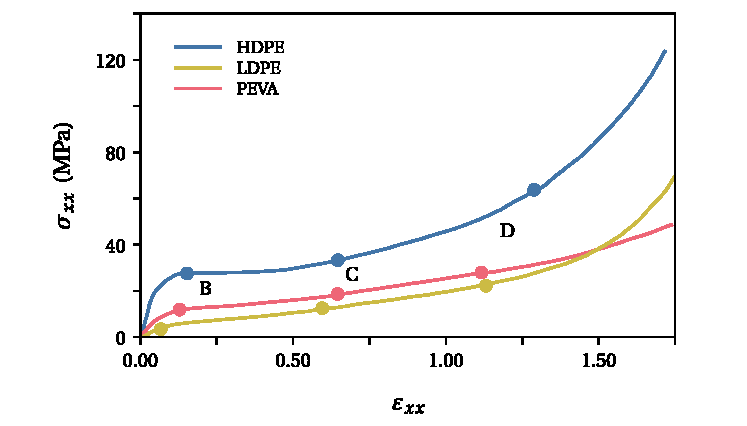
\includegraphics[width=\textwidth]{figures/stress_strain_curve_strobl}
	\caption{Locations of the transition points B-D along the stress-strain curve for HDPE, LDPE and PEVA. Adapted from \cite{hissNetworkStretchingSlip1999}.}
\label{fig:stress_strain_curve_strobl}
\end{figure}

\section{Mechanical response of semi-crystalline polymers}

The thermomechanical response of semi-crystalline polymers is reviewed in this section with the explicit goal of setting targets for constitutive modeling (see Chapter~\ref{ch:modeling_semi_crystalline_polymer} and \ref{ch:numerical_results}).
There are several factors affecting the mechanical response of semi-crystalline polymers.
Extrinsic factors, such as temperature, strain rate, hydrostatic pressure, and the chemical nature of the environment, e.g., the presence of water, oxygen, and organic solvents, are critical in describing the behavior of a polymer.
Other relevant elements in the characterization of semi-crystalline polymers are intrinsic.
Of crucial importance are the degree of crystallinity, lamellar thickness, mesoscopic structure, molecular weight, physical entanglement, cross-linking, and polymer aging \citep{ayoubEffectsCrystalContent2011, serbanTensilePropertiesSemicrystalline2013, callister2014materials, cundiffModelingViscoplasticBehavior2022}.

Numerous experimental procedures provide information about a material's mechanical response.
Constant strain rate tests are among the most relevant experiments for the characterization of semi-crystalline polymers, mainly through uniaxial loading experiments, whether tensile or compressive.
Pure shear and torsion tests are also employed.
Stress relaxation, creep experiments, and dynamic mechanical analysis are also necessary tests highlighting the material's time-dependent response.
The polymer's behavior upon unloading must also be considered, using step-cycle and free-shrinkage tests.
The information gathered from these last two experiments will aid in an appropriate discussion of the permanent deformation in semi-crystalline polymers, which is less readily defined than in most metals at room temperature.
The impact of the previously mentioned factors, such as temperature, strain rate, and hydrostatic pressure, on the mechanical response of the polymer in each type of experiment is thoroughly discussed in subsequent paragraphs.

\subsection{Constant strain rate loading}

The mechanical response of a semi-crystalline polymer in a constant strain-rate experiment is determined by several factors, as already mentioned; however, in the conditions typical for most applications, they exhibit the behavior of a plastic polymer.
These polymers exhibit structural rigidity under load and are suitable for general-purpose applications.
To be included in this material class, linear and branched polymers, if amorphous, must be used below their glass transition temperature, $T_g$, supposed to be in the range from \SI{100}{\celsius} to \SI{400}{\celsius} and much higher than their service temperature, $T_\mathrm{ser}$ or below their melting temperature if semi-crystalline \citep{callister2014materials, arzhakovRelaxationPhysicalMechanical2019}.

% \begin{figure}[hbtp]\
% 	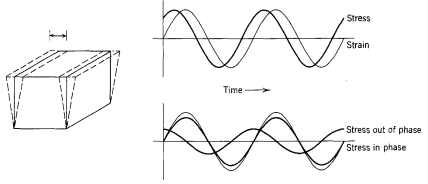
\includegraphics{mechanical_exp}
% 	\caption{Pure shear constant strain rate experiment.}
% \end{figure}

The stress-strain curves of plastic polymers consistently show a few basic features (see Figure~\ref{fig:response_plastic_polymer}).
The material exhibits a relatively stiff initial response, followed by yielding.
It must be stressed, however, that in most polymers, the development of permanent plastic strain is a continuous function of the applied strain, showing no discontinuity at the nominal stress drop or extrapolated yield point \citep{wardReviewYieldBehaviour1971} (see Remark~\ref{rmrk:yield_polymer}).
After this transient behavior, it sometimes follows a steady state where the stress stabilizes, after which strain hardening begins, intensifying dramatically at large strains \citep{hissNetworkStretchingSlip1999,callister2014materials,makradiTwophaseSelfconsistentModel2005}.
\begin{figure}[hbp]
	\centering
	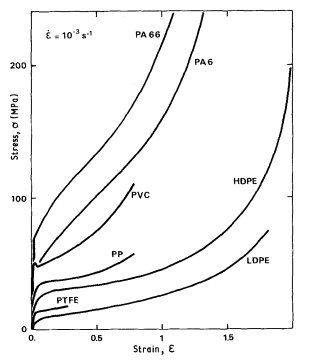
\includegraphics[width=0.9\textwidth]{figures/response_plastic_polymer}
	\caption{Stress-strain curves for different plastic polymers, including both glassy (PVC) and semi-crystalline (LDPE, HDPE, PTFE, PP, PA 6, PA 66) polymers in a constant strain rate uniaxial traction experiment. Adapted from \cite{gsellYieldTransientEffects1981}.}
\label{fig:response_plastic_polymer}
\end{figure}

\begin{remark}[Definition of yield in polymers]
YYielding is commonly defined as the beginning of plastic flow.
A common modeling assumption, employed, for example, when modeling metals far from their melting temperature, is that plastic flow only begins when a critical stress, the yield stress, is reached.
Polymers, on the other hand, present a more complex situation because, for many polymers, there may be flow, i.e., "yielding," at any stress level.
The initiation of plastic strain is mainly controlled by kinetic processes and appears to play no part in determining the yield stress of the material \citep{fotheringhamRoleRecoveryForces1978}, commonly defined in one of three ways: \citep{wardReviewYieldBehaviour1971}
	\begin{itemize}
		\item the stress at the maximum observed load;
		\item the stress corresponding to the point of intersection of two tangent lines on the stress-strain curve;
		\item the stress obtained when offsetting the linear portion of the response by a pre-defined strain amount.
	\end{itemize}
	See Figure~\ref{fig:yield_criteria} for the corresponding graphical depictions.
	\begin{center}
			\centering
								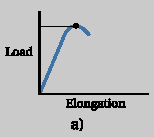
\includegraphics[width=0.3\textwidth]{figures/yield_criterion_a}
				\hfill
							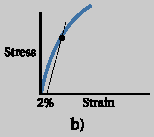
\includegraphics[width=0.3\textwidth]{figures/yield_criterion_b}
			\hfill
								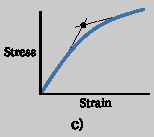
\includegraphics[width=0.3\textwidth]{figures/yield_criterion_c}
		\captionof{figure}{Yield criteria for polymers.}
		\label{fig:yield_criteria}
	\end{center}
\label{rmrk:yield_polymer}
\end{remark}

\paragraph{Pre-yield behavior}
Regarding the response of a semi-crystalline polymer pre-yield, an increase in temperature will lead to a more compliant response and a lower yield strength, as shown, in Figure~\ref{fig:scheme_effect_temperature} for nylon 101 \citep{khanThermomechanicalResponseNylon2006}, and in the results reported in \cite{brownInfluenceMolecularConformation2007} and \cite{hobeikaTemperatureStrainRate2000} for PEs.
In fact, the temperature is possibly the single most influential parameter dictating a polymer's mechanical response.
Some polymers may exhibit brittle fracture to necking or even homogeneous rupture during a uniaxial traction test depending on the temperature \citep{wardIntroductionMechanicalProperties2004}.
Moreover, whether the polymer is below or above its glass transition temperature results in markedly different behaviors in the case of amorphous polymers (see Figure~\ref{fig:scheme_effect_temperature} adapted from \cite{vanloockDeformationFailureMaps2018}).
An amorphous polymer in its glassy state behaves as a plastic polymer, whereas in its rubbery state, it has a much more compliant response, coinciding with very large deformations and a lack of a clear yield point.
On the other hand, even if the temperature of semi-crystalline polymer is much higher than its glass transition temperature, the crystalline phase causes the polymer's response to be qualitatively similar to that of a plastic polymer, although less stiff than it would be at a lower temperature (see Figure~\ref{fig:scheme_effect_temperature}).
\begin{figure}[hbtp]
	\centering
	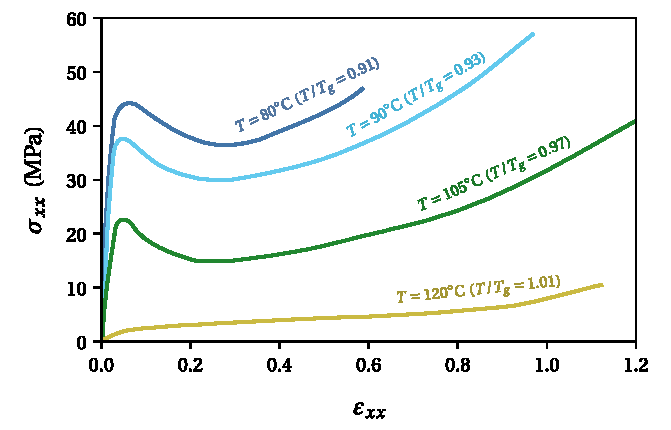
\includegraphics[width=0.9\textwidth]{figures/scheme_effect_temperature}
	\caption{Stress-strain curves for a semi-crystalline polymer (SCP), nylon 101 \citep{khanThermomechanicalResponseNylon2006}, and an amorphous polymer (AP), poly(methyl methacrylate) \citep{vanloockDeformationFailureMaps2018}, Above and below their glass transition temperatures, \SI{60}{\celsius} and \SI{118}{\celsius}, respectively.}
\label{fig:scheme_effect_temperature}
\end{figure}

The strain rate and the hydrostatic pressure, have the opposite effect, such that their increase will lead to a stiffer response and higher yield stresses, as gathered from the results in \cite{popelarViscoelasticMaterialCharacterization1990} (uniaxial traction) and \cite{trussEffectHydrostaticPressure1981} (torsion).
More specifically regarding the effect of the strain rate on the stress response, Walley and Field \citep{walleyStrainRateSensitivity1994} present experimental results for uniaxial compressive tests on a wide selection of polymers, including semi-crystalline polymers.
The HDPE samples display a linear relationship between the stress at different strain levels and the logarithm of the strain rate, while the PTFE's response shows a non-monotic relationship between the same quantities, which is however broadly increasing.
A linear relationhip between the maximum stress and the logarithm of the strain rate is found for PEEK, until a critical strain rate is reached, followed by a decrease in the stress response.
El-Qoubaa and Othman \citep{el-qoubaaStrainRateSensitivity2016} also provide an extensive set of results regarding the relationship between the strain rate, the temperature the yield strength of PEEK.
They find, however, that the yield stress of the polymer alway increases with the strain rate as shown in Figure~\ref{fig:el_qoubaa_peek}.
\begin{figure}[hbtp]
	\centering
	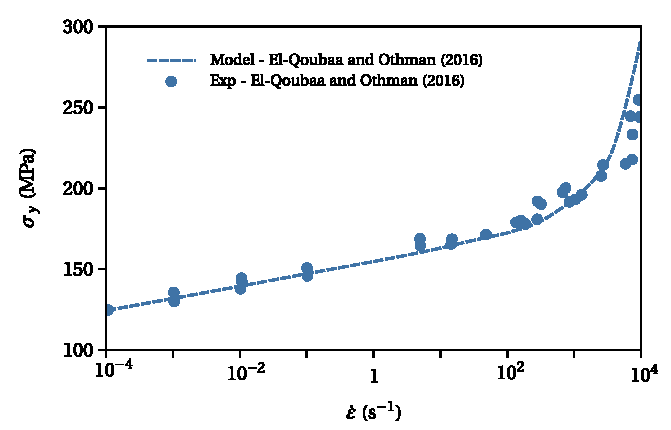
\includegraphics[width=0.9\textwidth]{figures/yield_el_qoubaa_peek}
	\caption{Yield stress, $\sigma_y$, as function of the strain rate, $\dot \varepsilon$, for PEEK at room temperature. Model and experimental results taken from \cite{el-qoubaaStrainRateSensitivity2016}.}
\label{fig:yield_el_qoubaa_peek}
\end{figure}


An increase in bulk crystallinity will lead to a stiffer response and increased strength as evident in the results of Ayoub et al. \citep{ayoubEffectsCrystalContent2011} and Bedoui et al. \citep{bedouiMicromechanicalModelingIsotropic2006} for polyethylenes with degrees of crystallinity by weight at room temperature ranging from 15 to 72\% (see Figure~\ref{fig:deg_cryst_stiff}).
However, the relationship between stiffness and crystallinity appears to be nonlinear.
\begin{figure}[hbtp]
	\centering
	\begin{subfigure}[b]{0.45\textwidth}
							\centering
							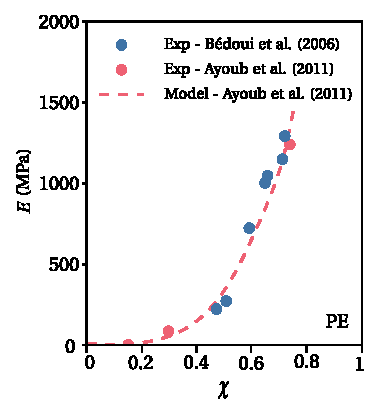
\includegraphics[width=\textwidth]{figures/deg_cryst_stiff}
							\caption{}
							\label{subfig:deg_cryst_stiff}
			\end{subfigure} \hfill
			\begin{subfigure}[b]{0.45\textwidth}
							\centering
							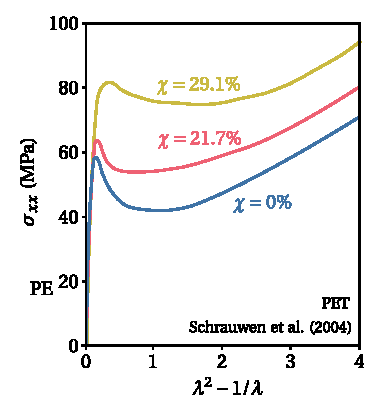
\includegraphics[width=\textwidth]{figures/deg_cryst_yield}
							\caption{}
							\label{subfig:deg_cryst_yield}
			\end{subfigure}
  \caption{Effect of the bulk crystallinity on \subref{subfig:deg_cryst_stiff} the Young modulus, $E$, and on the \subref{subfig:deg_cryst_yield} yield strength of a semi-crystalline polymer.}
\label{fig:deg_cryst_stiff}
\end{figure}
That said, Schrauwen et al. \citep{schrauwenIntrinsicDeformationBehavior2004} tests in uniaxial compression samples of both PET and PE containing more similar degrees of crystallinity among the samples, 0, 21.7, and 29.7\% and 68.4, 72.3, and 76.6\%, respectively, and no differences in the stiffness are visible in the results.
Clear increases, in the yield strength are, however, noticeable.
The results of Kurtz et al. \citep{kurtzThermomechanicalBehaviorVirgin2002} on UHWPE also support a positive correlation between the degreee of crystallinity and the stiffness as well as the yield strength.
The same authors \citep{kurtzMiniatureSpecimenMechanical1999, kurtzThermomechanicalBehaviorVirgin2002} also explore the effect of cross-linking due radiation combined with changes in crystallinity due to thermal treatments.
A decrease in the elastic modulus and the yield stress with the irradiation dose and the temperature of the thermal treatment is reported.

Schrauwen et al. \citep{schrauwenIntrinsicDeformationBehavior2004} further report that the yield stress is proportional to the lamellar thickness.
However, Argon \citep{argonPhysicsDeformationFracture2013a} mentions, based on results for PE, that this linear dependence is only observed for lamellae of conventional thickness in the range of \SIrange{10}{15}{\nano\meter}.
This dependence eventually breaks down with the yield strength remaining constant for thicknesses from \SIrange{20}{170}{\nano\meter}.
Also, for some polymers, an increase in molecular weigth leads to an increase in the their tensile strength.
This behavior is explained by an increase in chain entanglements with rising molecular weight \citep{callister2014materials}.

Regarding the effect of the mesostructure on the response of a semi-crystalline polymer, when comparing of the stress-strain curves of isotropic and oriented PE, the latter resists deformation more vigorously in the results concerning uniaxial traction presented in \cite{naViscousForceDominatedTensileDeformation2006}.

Finally, the critical strains at which the Hookean range ends or yield is observed are independent of the temperature and strain rate in the ranges considered by Hobeika et al. \citep{hobeikaTemperatureStrainRate2000}, i.e., \SIrange{23}{100}{\celsius} and \SIrange{10e-4}{10e-2}{\per\second}, in PE and PEVA.
In addition, both bulk crystallinity and molecular weight appear to have no impact in the location of these transition points.

\paragraph{Post-yield}
There may be some intrinsic strain softening after yielding, i.e., a decrease in stress with strain.
The results in \cite{schrauwenIntrinsicDeformationBehavior2004} show that after yield is reached, there is a sharp decrease in stress for completely amorphous PET above its glass transition temperature.
The drop becomes broader and less pronounced as crystallinity increases to values of 21.7 and 29.1\%.
The same authors present PE results that show no strain softening for a degree of crystallinity of 76.6\%.
Minor strain softening is visible at lower crystallinity values for the same polymer.
PP softens mildly as well, despite having a crystallinity of around 70\% in the samples studied.
These results were obtained under uniaxial compression, however, no softening is visible after yield in the results of Truss et al. \cite{trussEffectHydrostaticPressure1981} obtained for PE in torsion.
G'sell et al. \citep{gsellApplicationPlaneSimple1983} present results of pure shear experiments in which HDPE exhibit mild strain softening at \SI{23}{\celsius} while PP and PA66 show none.

The presence of strain softening can however change with the strain.
G'sell and Jonas \citep{gsellYieldTransientEffects1981} present the results of an experiment where the strain rate alternates between \SI{1e-3}{\per\second} and \SI{1e2}{\per \second}.
This makes possible the observation of stress transients at different strain levels, when the strain rate switches between the predetermined strain rates.
An unusual behavior is detected in semi-crystalline polymers below the glass transition temperature, such that for lower strains a "normal" transient, i,e,. corresponding to no strain softening, is observed, while at higher strains an "inverse" transient, i.e., coinciding with strain softening, is detected.
The latter type of transient is observable in glassy polymers when the same experiment is performed at any strain level.
The results of Nanzai \citep{nanzaiTransitionMechanismElastic1990} for poly(methyl methacrylate) (PMMA) support this claim regarding the transient behavior of glassy polymers.
According to G'sell and Jonas \citep{gsellDeterminationPlasticBehaviour1979}, an "inverse" transient happens when there are different conditions necessary for the initiation and the propagation of yielding.
Frost and Ashby \citep{frostDeformationmechanismMapsPlasticity1982} mention that such transients are observed in "hard" materials, where dislocations are not readly available, such as lithium floride crystals \citep{gilmanDislocationSourcesCrystals1959, johnstonYieldPointsDelay1962} or diamond \citep{alexanderDislocationsPlasticFlow1969}.

Despite the existence of intrinsic strain softening, its experimental observation is made difficult by two different phenomena: thermal softening and plastic instabilities.
The results presented thus far were obtained at strain rates slow enough to allow for isothermic evolution.
However, as the strain rate increases, a phenomenon known as temperature softening occurs, causing a similar decrease in stress with strain due to an increase in temperature.
This is rise in temperature is a result of the difficulty in offloading the heat generated by the plastic work in such a short period of time, making the process adiabatic.
According to Furmanski et al. \citep{furmanskiTimeTemperatureEquivalence2013}, this effect should be considered at strain rates greater than \SI{0.01}{s^{-1}} and strains greater than 15\%.
Cundiff et al. \citep{cundiffModelingViscoplasticBehavior2022}, for example, reports uniaxial compressive tests for PA 6 where temperature induced strain softening may be observed.

Plastic instabilities, i.e., the growth of a locally thinned region in a material upon application of stresses, must also be considered when the intrinsic response of the material is sought.
They are a function of the geometry and loading conditions of the loaded body, in addition to its intrinsic constitutive behavior \citep{wardIntroductionMechanicalProperties2004}.
While uniaxial compressive loading, in general, doesn't lead to heterogeneous deformation, this is not the case for uniaxial traction experiments, which often, but not always, lead to necking (see the comparison between isotropic and oriented PE in \cite{naViscousForceDominatedTensileDeformation2006}), or simple shear experiments, which may lead to shear banding \citep{gsellApplicationPlaneSimple1983}.
There are however experimental methods which allow for the use of uniaxial traction tests in the determination of intrisic material behavior.
The video-controlled technique in \citep{gsellVideocontrolledTensileTesting1992} is one example, as is the SEÉ method \citep{lauroSEEMethodDetermination2010, balieuDamageHighStrain2015} which uses the full-field data from digitial correlation measurements of heterogeneous displacement fields.

For a material whose stress response depends only on the strain, a maximum in the nominal stress implies the formation of a neck \citep{wardIntroductionMechanicalProperties2004}.
There are also other equivalent criteria, such as Considère's criterion for necking.
Polymers, however, exhibit a strain rate dependence and thus, because necking is associated with a local increase in strain rate, a strong such dependence, can inhibit necking even when the nominal stress reaches a maximum.
For these materials, the existence of a maximum in the nominal stress is only a necessary condition \citep{wardIntroductionMechanicalProperties2004}.
In fact, according to Brooks et al. \citep{brooksModelingDoubleYield1995}, a double yield phenomenon is observed in polyethylenes ranging from LDPE to HDPE.
Lucas et al. \cite{lucasDoubleYieldTensile1995} report similar results for linear polyethylenes and well-characterized ethylene copolymers of narrow molecular weight and composition distributions.
Hao et al. \citep{haoRatedependentConstitutiveModel2022} mention that this phenomenon has also been observed on polyamide (PA), polytrimethyleneterephthalate (PTT) and polybutyleneterephthalate (PBT).
The force maximum observed at the first yield point under certain conditions is therefore to be associated with a homogeneous strain-softening process within the materials and not with the development of the neck (i.e., a geometrical instability) which occurs at the second yield point (see Figure~\ref{fig:double_yield}).
These experimental results make clear that such complex yielding processes are not always observed, being more likely to occur with low crystallinity ratios and low strain rates \citep{zengConstitutiveModelSemicrystalline2010}.
\begin{figure}[htbp]
	\centering
	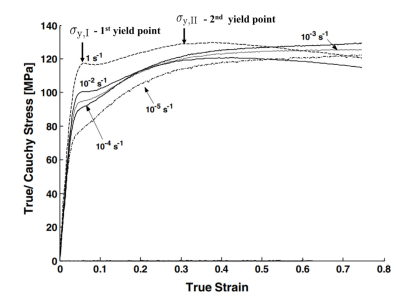
\includegraphics[width=0.9\textwidth]{figures/double_yield}
	\caption{Stress-strain curve for polyethylenes exhibiting double yield. Adapted from \cite{khanThermomechanicalResponseNylon2006}.}
\label{fig:double_yield}
\end{figure}

\cite{yeKinematicStudyNecking2015} reports that for HDPE even with measurements made on a relatively small strain rate range (smaller than 1 decade), the necking phenomenon depends on the strain rate.
In particular, they found that, around the yield point, the strain localization is more pronounced with higher strain rates.

After necking occurs—usually at the maximum load, but not always, as in the case of double yield—the material resists by reorienting the polymer chains, so that the deformation is not limited to the necking zone, as in ductile materials \citep{callister2014materials}.
As the specimen thins from the initial cross-section to the drawn cross-section, the shoulders of the neck travel along it, in what is called cold drawing (see Figure~\ref{fig:natural_draw_ratio}).
The existence of a finite or natural draw ratio, i.e., a strain deformation corresponding to the stable propagation of the neck, is an important aspect of polymer deformation because a stabilized neck is not always formed \citep{wardIntroductionMechanicalProperties2004}.
The neck's stable propagation occurs when the neck area has hardened sufficiently, allowing other sections of the specimen to meet the necking criteria.
If this is the case, Considéré's criterion for necking can be used to determine it.
\begin{figure}[hbtp]
	\centering
	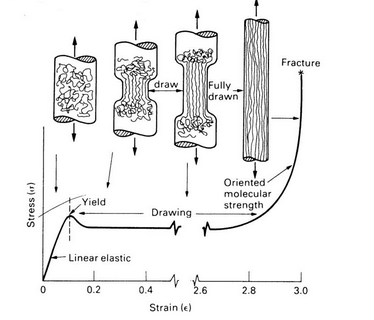
\includegraphics[width=0.9\textwidth]{figures/natural_draw_ratio}
	\caption{Schematic depiction of two uniaxial traction experiments. One where there is formation of a neck and stabilization, corresponding to cold drawing, and the other with neck formation and no neck stabilization, such that cold drawing is not observed.}
\label{fig:natural_draw_ratio}
\end{figure}

Another important aspect regarding the plasticity of semi-crystalline polymers is that, in contrast to metals, permanent volumetric strains can be detected in addition to elasticity-related volumetric strains.
These effects found both in tension and compression cannot be explained by Hooke's elasticity and correspond to an irreversible contraction or dilation of the material \citep{cangemiTwoPhaseModelMechanical2001,polanco-loriaConstitutiveModelThermoplastics2010}.

Cangemi and Meimon \citep{cangemiTwoPhaseModelMechanical2001} report the existence of plastic dilation in compression for semi-crystalline polymers.
In contrast, for glassy polymers show a very weak contraction.
According to the same authors' results for PA11, the effect of plasticity on volumetric strain is felt when a strain of \num{0.03} is reached.
Until then, the material contracts, after which a significant volume increase is observed.
An increase in confining pressure was also investigated, and the authors discovered that it resulted in a qualitatively similar evolution of the volumetric strain, though it was more pronounced in magnitude, before attaining approximately the same value after a strain of \num{0.16} is reached.
Tensile tests were also performed by the authors, during which the volume strain increases globally, due to the elastic response of the material.
As the material approaches the plastic domain, the total volume strain reduces slightly and then increases again at the end of the test.
Qualitatively identical results were obtained by other authors for PA11 \citep{marchalInfluenceCheminChargement1996}.

Damage, or void growth, is one obvious mechanism responsible for these observations.
However, Polanco-Loria et al. \citep{polanco-loriaConstitutiveModelThermoplastics2010} mention that an increase in volume in semi-crystalline polymers may also be associated with crystalline deformation.
This is because in the crystalline phase the molecules are organized in a rather dense manner, thus the specific volume is likely to increase when the crystalline lamellae break up.
In fact, after a compression test in which the specimens showed net plastic expansion for the majority of the test, Kitagawa and Yoneyama \citep{kitagawaPlasticDilatationDue1988} made thin cuttings of semi-crystalline polymer samples (PP, POM, and PE) for observations in a polarized light microscope.
There were no cracks or crazes found.
This point expresses the peculiarity of plastic volume expansion in semi-crystalline polymers, which may be related to the complexity of their microstructures as well as their two phase nature \citep{cangemiTwoPhaseModelMechanical2001}.

\paragraph{Steady state flow}

After the transient described is cleared and before strain hardening starts to become noticeable there is a period of steady state flow, in which the polymer flows at constant stress function of the temperature and the strain rate.
Both Kurtz et al. \citep{kurtzThermomechanicalBehaviorVirgin2002}, for UHWPE, and G'sell and Jonas \citep{gsellDeterminationPlasticBehaviour1979}, for HDPE, found a reduced strain rate dependendence coinciding with a small coefficient fiting a power law relationship between the stress and the strain rate comparable to metals.
The first authors point out, however, based on their results for UHWPE, that the strain rate sensitivity increases significantly with temperature.

\paragraph{Strain hardening}
Semi-crystalline polymers, if ductile enough, will exhibit strain hardening, which can be quite dramatic at higher strains.
Orientation hardening at large deformation due to molecular alignment is the main source of strain hardening \citep{ahziModelingDeformationBehavior2003}.
In addition to molecular alignement, crystal orientation may also contribute to the strain hardening observed in semi-crystalline polymers \citep{abdul-hameedTwophaseHyperelasticviscoplasticConstitutive2014}.

The results presented by G'Sell and Jonas \citep{gsellYieldTransientEffects1981} at constant strain rate clearly show that at \SI{22}{\celsius} and a strain rate of \SI{1e-3}{\per\second} semi-crystalline polymers such as HDPE, LDPE, PA6 and PA66 show marked strain hardening.
Based on the previously mentioned compressive tests, Schrauwen et al. \citep{schrauwenIntrinsicDeformationBehavior2004} conclude that crystallinity and lamellar thickness have no effect on the strain hardening of semi-crystalline polymers, however the melt cooling procedure and subsequent heat treatments do.
This suggests that the mesostructure may have an effect on the polymer's strain hardening behavior.

\paragraph{Failure}
The maximum strain at rupture for semi-crystalline polymers can be very large, as evidenced by the results of G'Sell and co-workers \citep{gsellYieldTransientEffects1981, gsellApplicationPlaneSimple1983}.
HDPE can reach strains of more than 2 in tensile tests and more than 10 in shear tests.
This is significantly greater than what glassy polymers like PVC and PC can achieve.

\paragraph{Experimental results}

Table~\ref{tab:exp_res_cnst_strain_rate} compiles a sample fo the available experimental results in the literature concerning constant strain rate experiments on semi-crystaline polymers.

\begin{landscape}
\begin{table}[!ht]
\caption{Experimental results concerning constant strain rate experiments.}
\label{tab:exp_res_cnst_strain_rate}
		\small
    \centering
		% \sisetup{range-phrase=--, round-mode=places, round-precision=1, table-format = 1.2e1, table-number-alignment =center, table-figures-exponent=1}
    \begin{tabular}{
		l
		S[round-mode=places, round-precision=0, table-format = 1e1]
		c
		c
		c
		l
		p{8em}
		% p{3em}
		}
		\hline
        Author\vphantom{\Big |} & {Strain rate (\si{\per\second})} & Temperature (\si{\celsius}) & Pressure (\si{\mega\pascal})  & Max strain & Loading mode & Material
				% & Obs
				\\ \hline \hline
        \cite{gsellYieldTransientEffects1981}\vphantom{\Big |} & \SIrange{2e-4}{.9e-1}{} & 22 & Ambient & 1.5 - 2 & Uniaxial traction & HDPE
				% & Transient dip and relaxation-reload curves also included.
				\\
        \cite{gsellYieldTransientEffects1981} & 1e-3 & 22 & Ambient & 1.7 & Uniaxial traction & LDPE, HDPE, PA6, PA66, PTFE
				% & Transient dip and relaxation-reload curves also included.
				\\
        \cite{trussEffectHydrostaticPressure1981} & 9.4e-4 & 20 & \SIrange{1e-1}{4e2}{} & 0.16 & Torsion & Rigidex xxx
				% & ~
				\\
        \cite{popelarViscoelasticMaterialCharacterization1990} & \SIrange{1e-5}{1e-1}{} & 23, 77 & Ambient & 0.25 & Uniaxial traction & MDPE, HDPE
				% & Includes unloading
				\\
        \cite{gsellEvolutionMicrostructureSemicrystalline1994} & 5e-4 & 25 & Ambient & 2 & Uniaxial traction & HDPE
				% & Includes also shear
				\\
        \cite{hissNetworkStretchingSlip1999} & \SIrange{1e-4}{1e-2}{} & Room & Ambient & 2 & Uniaxial & HDPE
				% & ~
				\\
        \cite{hissNetworkStretchingSlip1999} & 5e-3 & Room & Ambient & \SIrange{1.75}{2}{} & Uniaxial traction & HDPE, LDPE, PEVA
				% & Step-cycle tests are also presented.
				\\
        \cite{hobeikaTemperatureStrainRate2000} & \SIrange{1e-4}{1e-2}{} & \SIrange{23}{110}{} & Ambient & 1.8 & Uniaxial traction & HDPE, LDPE, PEVA
				% & The strain split is also analysed.
				\\
        \cite{beijerModellingCreepBehaviour2000} & \SIrange{3.16e-7}{1e-1}{} & 43 & Ambient & 0.25 & Uniaxial & HDPE
				% & ~
				\\
        \cite{schrauwenIntrinsicDeformationBehavior2004} & 3e-3 & Room & Ambient & 0.9 & Uniaxial compression & PE
				% & Comparison between samples with different crystallinity and lamellar thickness.
				\\
        \cite{naViscousForceDominatedTensileDeformation2006} & \SIrange{1e-3}{1e-2}{} & Room & Ambient & 1 & Uniaxial & Oriented HDPE
				% & Step-cycle tests are also included.
				\\
        \cite{drozdovFiniteViscoelasticityViscoplasticity2007} & \SIrange{5e-4}{3e-2}{} & Room & Ambient & 0.2 & Uniaxial traction & LDPE
				% & Tensile
				\\
        \cite{drozdovFiniteViscoelasticityViscoplasticity2007} & \SIrange{5e-4}{1e-1}{} & Room & Ambient & 0.2 & Uniaxial compression & LDPE
				% & ~
				\\
        \cite{brownInfluenceMolecularConformation2007} & \SIrange{1e-4}{2.6e3}{} & \SIrange{-75}{100}{} & Ambient & 0.5 & Uniaxial compression & HDPE, PEX, UHWPE
				% & ~
				\\
        \cite{ayoubModellingLargeDeformation2010} & \SIrange{5e-4}{1e-2}{} & Ambient & Ambient & 2.5 & Uniaxial & HDPE
				% & Includes reloading at different prestrains
				\\
        \cite{zengConstitutiveModelSemicrystalline2010} & \SIrange{2.77e-2}{1.11e-1}{} & 90 & Ambient & 1.5 & Uniaxial traction & PE, PA6
				% & Tensile; includes reloading at different prestrains. Biaxial results are also included.
				\\
        \cite{ayoubEffectsCrystalContent2011} & \SIrange{1e-4}{1e-2}{} & Ambient & Ambient & 1.8 & Uniaxial traction & PE copolymers
				% & Each material has different crystallinity (15\% to 72\%)
				\\
        \cite{furmanskiTimeTemperatureEquivalence2013} & \SIrange{1e-3}{1}{} & \SIrange{-80}{20}{} & Ambient & 0.6 & Uniaxial compression & HDPE, UHMWPE
				% & ~
				\\
        \cite{bergstromMechanicsSolidPolymers2015} & \SIrange{2e-3}{1e-2}{} & - & Ambient & 0.5 & Uniaxial traction & PTFE \\
        \cite{bergstromMechanicsSolidPolymers2015} & \SIrange{2e-4}{2e-2}{} & - & Ambient & 0.35 & Uniaxial & HDPE
				% & ~
				\\
        \cite{ariebyAnisotropicMechanicalBehavior2017} & 1e-3 & Ambient & Ambient & 1.6 & Uniaxial traction & HDPE
				% & Volumetric strain included. Anisotropy also studied.
				\\ \hline \hline
    \end{tabular}
\end{table}
\end{landscape}

\subsection{Stress relaxation, creep  and dynamic mechanical analysis experiments}
\label{sec:relax_creep_dma}

The stress relaxation, creep and dynamic mechanical analysis experiments are all pertinent experiments to characterize the time-dependent behavior of a material.
In particular, the semi-crystalline polymers exhibit a time-dependent behavior that sets them apart, for example, from metals at temperatures far below their melting point.
This section will first focus on isothermic measurements, then on isochronal measurements.

The stress relaxation experiment involves applying a constant strain to the material.
Typically for polymeric systems, the resulting stress response, that is, the so-called relaxation modulus, decreases with time.
A sharp drop is however not noticeable in highly semi-crystalline and glassy polymers, which exhibit stress relaxation moduli in the order of gigaPascals, as depicted in Figure~\ref{subfig:relax_modulus_scp}.
Semi-crystalline polymers with a lower crystalline content exhibit a primary viscoelastic transition from a glasslike to a leathery consistency as a decrease in the stiffness from the order of \SIrange{10e9}{10e7}{\pascal}, as shown in Figure~\ref{subfig:relax_modulus_scp}.
These polymer with a degree of crystallinity between ~5 to 10\% are termed by Tobolsky \citep{tobolskyPropertiesStructurePolymers1960} as very slightly crystalline polymers.
This is similar to the behavior of cross-linked amorphous polymers, since individual molecules may thread in and out of crystalline regions which act as multiple cross-links \citep{ferryViscoelasticPropertiesPolymers1980, gsellYieldTransientEffects1981}.
See, for example, the results of Faucher \citep{faucherViscoelasticBehaviorPolyethylene1959} comparing the relaxation behavior of amorphous and crystalline polypropylene.


This change in the material's response with time is commonly referred to as a transition from a glasslike to a rubberlike (or leatherlike, if a stiffer response is observed) behavior.
However, it is a viscoelastic transition, not the transition verified at the glass transition temperature in which the thermodynamic state of the material changes.
The thermodynamical state of the material remains unchanged in this case, with this particular behavior traceable to the manner in which the kinetic units flow.
Their flow can be described as a thermally activated process where the energetic barriers preventing their motion are cleared with the help of random thermal fluctuations.
The kinetic units have to "wait" until a large enough thermal variation puts them over the hump and they begin moving.
Thus, for very short times the response of the material will be stiffer, as the kinetic units do not have enough time to flow.
As time goes on more and more kinetic units will be able to move leading to a softer response.
Hence, in time dependent materials, the ratio of the time it takes for a material to adjust to applied stresses or deformations, the relaxation time, $t_c$, and the characteristic time scale of an experiment (or a computer simulation), $t_p$, probing the response of the material is especially important.
The Deborah number is the dimensionless quantity defined as this ratio, such that flow will happen when \citep{wardIntroductionMechanicalProperties2004, arzhakovRelaxationPhysicalMechanical2019}
\begin{equation}
	\mathrm{De}=\frac{t_c}{t_p}\approx 1\text{, or  }t_c\approx t_p.
\end{equation}

A constant stress is imposed in a creep experiment, for example, by dead-loading \citep{wildingCreepRecoveryUltra1981}, and an increase in strain is expected over time.
This strain response is the so-called creep compliance of the material.
Glassy polymers and highly crystalline polymers exhibit similar behaviors, with very slow increases in creep compliance with time at the longest times of observation, as do low crystallinity polymers and crosslinked polymers, which exhibit a viscoelastic transition via an increase in compliance as time progresses \citep{ferryViscoelasticPropertiesPolymers1980} (see Figure~\ref{subfig:creep_compliance_scp}).
\begin{figure}[hbtp]
	\centering
	\begin{subfigure}[b]{0.45\textwidth}
							\centering
							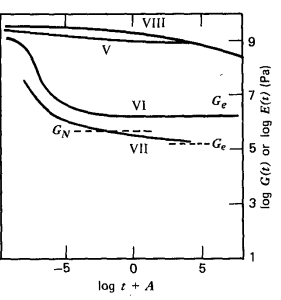
\includegraphics[width=\textwidth]{figures/relax_modulus_scp}
							\caption{}
							\label{subfig:relax_modulus_scp}
			\end{subfigure} \hfill
			\begin{subfigure}[b]{0.45\textwidth}
							\centering
							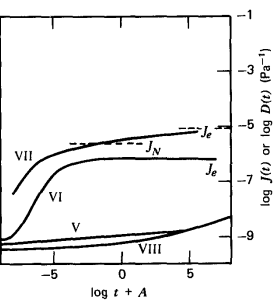
\includegraphics[width=\textwidth]{figures/creep_compliance_scp}
							\caption{}
							\label{subfig:creep_compliance_scp}
			\end{subfigure}
	\caption{Typical viscoelastic properties of a very lightly crosslinked polymer (I), slightly crystalline or lightly crosslinked polymer (II), glassy polymer (III) and highly crystalline polymer. \subref{subfig:relax_modulus_scp} relaxation modulus, $G$. \subref{subfig:creep_compliance_scp} creep compliance, $J$. $A$ is an appropriate horizaontal shift constant. Adapted from \cite{ferryViscoelasticPropertiesPolymers1980}.}
\label{fig:relax_creep_scp}
\end{figure}

A dynamic mechanical analysis (DMA) employs either a strain or stress driven steady state harmonic oscillation and records the corresponding stress or strain response, respectively.
For a strain driven experiment, the quantities of interest are the storage and loss moduli, defined as the stress response in phase and out phase relative to the strain divided by the strain amplitude, and the loss tangent, which is the tangent of the phase shift between the strain and the stress.
The loss and storage compliances can be defined in a similar way when considering a stress driven experiment.
Their physical interpretation is suggested by their respective names, as they are measures of the energy stored and lost per cycle.
For a perfectly elastic material one would expect no loss, and thus for the stress and the strain to be in phase.
On the other hand, a completely viscous material would exhibit a 90° degree phase shift, dissipating all the energy supplied to the system as heat.
A real material will display an intermediate behavior depending on the frequency.
When $\omega\ t_c \approx 1$, i.e., $\mathrm{De} \approx 1$, for some deformation mechanism with a relaxation time of $t_c$, there will be an increase in the viscous character of the material, hence leading to a drop in  the storage modulus, and maxima in loss modulus and loss tangent (often, not exactly at the same frequency) \citep{ferryViscoelasticPropertiesPolymers1980}.

The storage modulus and compliance are approximately mirror images of the stress relaxation modulus and creep compliance, since a dynamic measurement at frequency $\omega$ is qualitatively equivalent to a transient one at $t=1/\omega$.
The glassy and crystalline polymers have values in the general neighborhood of 0.1 for the tangent loss, and may present several maxima associated with various deformation mechanisms \citep{ferryViscoelasticPropertiesPolymers1980}.
See Figure~\ref{fig:dma_scp} for the loss and storage modulus of highly and lightly crystalline polymers.
\begin{figure}[hbtp]
\centering
\begin{subfigure}[b]{0.45\textwidth}
\centering
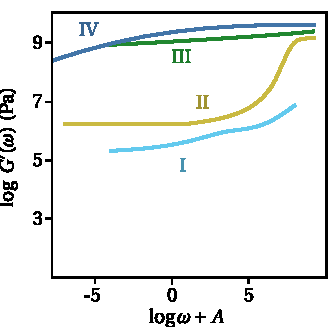
\includegraphics[width=\textwidth]{figures/storage_modulus_scp}
\caption{}
\label{subfig:storage_modulus_scp}
\end{subfigure} \hfill
	\begin{subfigure}[b]{0.45\textwidth}
		\centering
						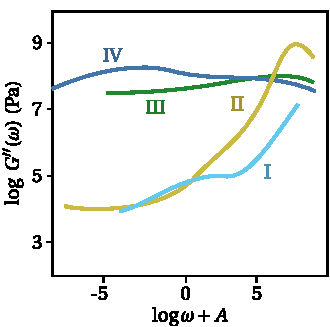
\includegraphics[width=\textwidth]{figures/loss_modulus_scp}
						\caption{}
						\label{subfig:loss_modulus_scp}
		\end{subfigure}
	\caption{Typical viscoelastic properties of a very lightly crosslinked polymer (I), slightly crystalline or lightly crosslinked polymer (II), glassy polymer (III) and highly crystalline polymer. \subref{subfig:relax_modulus_scp} storage modulus, $G^\prime$. \subref{subfig:creep_compliance_scp} loss modulus, $G^{\prime\prime}$. $A$ is an appropriate horizaontal shift constant. Adapted from \cite{ferryViscoelasticPropertiesPolymers1980}.}
\label{fig:dma_scp}
\end{figure}

Ferry \citep{ferryViscoelasticPropertiesPolymers1980} collects some experimental results illustrating the nonlinear behavior of semi-crystalline polymers.
For a more thorough discussion on what is the expected linear behavior for a time-dependent material see Section~\ref{sec:infinitesimal_thermo_viscoelasticity}.
In a stress relaxation experiment, a linear behavior implies coinciding curves when the relaxation modulus divided by the strain is ploted for different strains levels.
However, for tensile stress relaxation of PE single crystal mats, the ratio of stress to strain decreases more rapidly with time at higher extensions, in the range of $\epsilon = \SIrange{0.0003}{0.003}{}$; the degree of nonlinearity increases markedly with decreasing temperature in the range of \SIrange{40}{10}{\celsius}.
Nonlinear creep recovery of polyethylene has also been reported.
It is demonstrated that after a partial stress relaxation at constant strain for various times and strain magnitudes, recovery is much slower at large strains but somewhat faster for shorter durations of the initial straining.
In this system, strains less than 0.01\% appear to be required for a linear behavior.
Nonlinear behavior when subject to sinusoidal deformations with large amplitudes has also been investigated.
Finally, Ben Hadj Hamouda et al. \citep{benhadjhamoudaViscoplasticBehaviourMedium2007} report the existence of two regimes of creep deformation for medium density ethylene-butene copolymer (MDPE).

\begin{remark}[Types of non-linear behavior]
	AAccording, to Malkin \citep{malkinNonlinearityRheologyEssay1995} there are three types of non-linearity in the constitutive response of a material.
	\begin{enumerate}
		\item \textit{geometrical, stationary or weak non-linearity:} characterized by permanent material constants and unchanging relaxation properties. The neo-Hookean behavior of rubbers is one such example;
		\item \textit{physical, kinetic or strong non-linearity:} explained by changes in the inherent structure of a material due to deformation and characterized by changing material constants and relaxation properties with deformation. The hysteresis in repeated deformations of rubbers (Mullins effect) and crystalline polymers;
		\item \textit{phase, thermodynamic or rupture non-linearity:} explained by phase or relaxation transitions induced by deformation and characterized by change in the physical state of the material and radical changes in its relaxation spectrum. The transition of linear polymers from a rubbery to a glassy state is one example.
	\end{enumerate}
\end{remark}

The results previously discussed were obtained at a constant temperature, and are thus isothermal.
Running the tests at different temperatures it is often possible to extend the time/frequency range of the experimental results employing the method of reduced variables, also known as the time-temperature superposition principle, or the thermorheological simple postulate \citep{ferryViscoelasticPropertiesPolymers1980, christensen2013theory}.
It consists in an appropriate horizontal and vertical shift of experimental results obtained at different temperatures to construct a single isothermal master curve.
A physical justification for the applicability of this procedure regarding the horizontal shift can be given in terms of the thermally activated processes that underlie the deformation mechanisms responsible for the relaxation transitions \citep{arzhakovRelaxationPhysicalMechanical2019}
There are several models for the horizontal shift, perhaps the most well known being the site model theory and the Williams, Landel and Ferry (WLF) equation \citep{wardIntroductionMechanicalProperties2004, furmanskiTimeTemperatureEquivalence2013}
A more detailed discussion of the models is given in Section~\ref{sec:viscous_elements}.
A suitable vertical shift can be achieved through the multiplication by $T_0\rho_0/T\rho$, where the subscript 0 denotes a reference state and $T$ and $\rho$ are the temperature and the density, respectively.
Its use is justified due to the entropy-spring nature of the stored elastic energy in the flexible chain theory \citep{ferryViscoelasticPropertiesPolymers1980}.
An application of the time-temperature superposition principle can be found in \cite{popelarViscoelasticMaterialCharacterization1990}, where a master curve is built for a polyethylene employing both horizontal and vertical shifts.

Isochronal results are obtained when the mechanical experiments described in this section are performed at different temperatures and plotted for the same time or frequency.
These are in fact the most common type of available data on semi-crystalline polymers \citep{ferryViscoelasticPropertiesPolymers1980}.
It should be noted that the system's structure changes with temperature, and thus an isothermal plot is, in some respects, more closely and simply related to the distribution of relaxation times than an isochronal plot \citep{hoffmanAnalysisRelaxationsPolychlorotrifluoroethylene2007}.
For example, there are relaxation behaviors that cannot be measured in low crystallinity samples of PCTFE, as it begins to crystallize before the corresponding temperature is reached \citep{hoffmanAnalysisRelaxationsPolychlorotrifluoroethylene2007}.

Focus is given here to results obtained through DMA, although most observations apply to stress relaxation results as well as creep results.
The most important information gathered from these experiments is the temperature of the relaxation transition at a given frequency.
Starting with low crystallinity polymers helps clarify the discussion of relaxation transitions in semi-crystalline polymers.
In fact, for a completely amorphous polymer glass, there will be two important transitions: the alpha and beta transitions.
The alpha transition is tightly connected to the glass transition\footnote{The glass transition is a thermodynamic transition which also implies a structure change in terms of a decrease in the free volume in addition to the cooperative motion of the polymer molecules associated with the alpha viscoelastic transition}, and it is the main viscoelastic transition, while the beta transition is another transition happening generally at a lower temperature \citep{arzhakovRelaxationPhysicalMechanical2019}.
Which of these happens at higher temperature may change at high enough frequencies \citep{matsuokaThermodynamicTheoryViscoelasticity1996}.
According to Arzhakov \citep{arzhakovRelaxationPhysicalMechanical2019}, the elementary kinetic unit responsible for these transitions is a macromolecule segment, with the beta transition being linked to the quasi-independent, localized displacement of the segments (intramolecule), and the alpha transition, to these quasi-independent modes acquiring a cooperative, coorelated character (intermolecule) \citep{bershteinGeneralMechanismTransition1985, matsuokaThermodynamicTheoryViscoelasticity1996}.
As the extent of crystallinity decreases and amorphous domains large enough to allow configurational rearrangements of longer chain segments appear in semi-crystalline polymers, the motions responsible for these two transitions presumably gradually resemble those seen in the amorphous state in the transition zone of viscoelastic behavior \citep{ferryViscoelasticPropertiesPolymers1980}.

The previously used notation for alpha and beta transitions applies only to amorphous polymers.
In general, semi-crystalline polymer transitions are also classified using the Greek alphabet, but without taking into account the character of the molecular motions corresponding to the transition or the phase in the polymer where it occurs.
The transitions are named alphabetically beginning with alpha in descending order of temperature, resulting in a sometimes confusing literature in which naming is not standardized.
Here, the naming convention will follow the suggestion in \cite{arzhakovRelaxationPhysicalMechanical2019}, using increasing Roman numerals for relaxations verified at increasing temperatures.

Starting at the lowest temperatures, increasing the crystal content of the polymer has little effect on the temperature at which the Relaxation I is verified, resulting in similar loss moduli and loss tangent profiles.
See the results for:
\begin{itemize}
	\item PET ($\beta$ relaxation) by Takayanagi presented in \cite{wardIntroductionMechanicalProperties2004} with degrees of crystallinity of 5, 34 and 50\%, corresponding to \SI{-60}{\celsius} at \SI{138}{\hertz};
	\item for PCTFE ($\gamma$ relaxation) in \cite{mccrumVariationInternalFriction1962} with degrees of crystallinity of 27, 42 and 80\%, corresponding to \SI{-40}{\celsius} at \SI{1}{\hertz};
	\item for PE in \cite{khannaDynamicMechanicalRelaxations1985} with degrees of crystallinity of ~50\% (LDPE) and ~65\% (HDPE), corresponding to \SI{-110}{\celsius} at \SI{1}{\hertz};
	\item for PP in \cite{mccrumStudyInternalFriction1959} with different unspecified degrees of crystallinity, corresponding to \SI{-30}{\celsius} at \SI{1}{\hertz}.
\end{itemize}

However, the temperature at which the next transition, Relaxation II, is verified varies with crystallinity.
For example, for the PE samples studied in \cite{khannaDynamicMechanicalRelaxations1985}, it varied between \SI{-27}{\celsius} and \SI{-10}{\celsius}.
With increasing crystallinity, this relaxation becomes broader and less pronounced.
Relaxation I and II happen in the bulk amorphous phase of the semi-crystalline polymers and the corresponding motions of the kinetic units are the ones responsible by the $\beta$ and $\alpha$ transitions in the completely amorphous polymers.
The disappearance of the relaxations II with the increase in crystallinity is tied to the shrinking of the amorphous domains, and decrease in the number of longer kinetic units responsible for the relaxation.
On the other hand, the relaxations I are connected to motions of smaller kinetic units like the $\beta$ transition in the amorphous polymers, and hence are not affected in the same way by the increase in crystallinity.

The appearance and increase in the size of the crystalline phase will lead to the appearance of a third transition, Relaxation III, at higher temperatures.
This transition is connected to motions on the surface of the crystal lamellae, and the temperature at which is verified vary with their thickness \citep{khannaDynamicMechanicalRelaxations1985, hoffmanAnalysisRelaxationsPolychlorotrifluoroethylene2007}.
Hoffman et al. \citep{hoffmanAnalysisRelaxationsPolychlorotrifluoroethylene2007} present a detailed model of the motions connected to each of the transitions in PCTFE and PE.
Ward and Sweeney \citep{wardIntroductionMechanicalProperties2004} also provide an explanation based on the deformation mechanism available with increasing crystallinity for the "disappearance" of Relaxation II in PE.

According to Arzhakov \citep{arzhakovRelaxationPhysicalMechanical2019}, employing etching techniques that remove the amorphous phase, it can be gathered that the relaxation transitions described so far originate in kinetic units found in the amorphous phase of the polymer.
There is however sometimes a fourth relaxation, connected to the kinetic units in the crystalline phase, and may imply the melting of some of the crystallites.
This transition appears to be visible in the results of Panowicz et al. \citep{panowiczPropertiesPolyethyleneTerephthalate2021} for PET.
It seems, however, not to be noticeable in the other experimental results mentioned so far.
Hoffman et al. \citep{hoffmanAnalysisRelaxationsPolychlorotrifluoroethylene2007} also mention the existence of a cryogenic transition, present in some polymers, such as isotactic propylene (iPP).

\begin{figure}[htbp]
\centering
\begin{subfigure}[b]{0.45\textwidth}
\centering
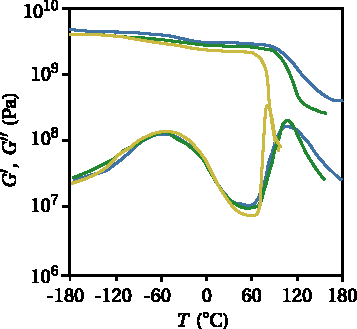
\includegraphics[width=\textwidth]{figures/pet_dma}
\caption{}
\label{subfig:pet_dma}
\end{subfigure} \hfill
	\begin{subfigure}[b]{0.45\textwidth}
		\centering
						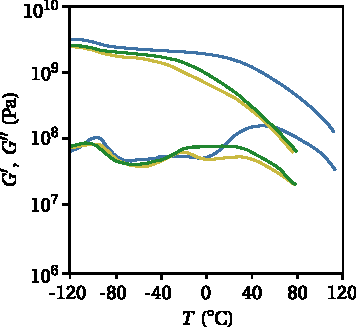
\includegraphics[width=\textwidth]{figures/pe_dma}
						\caption{}
						\label{subfig:pe_dma}
		\end{subfigure}
	\caption{title}
\end{figure}

As an example of a semi-crystalline polymer that doesn't fit exactly into the classification scheme just provided see the results of McCrum \cite{mccrumStudyInternalFriction1959} for PTFE with crystallinities ranging from 48 to 92\%.
The relaxation observed at the lower temperatures ($\approx$\SI{-100}{\celsius}) disappears with the increase in crystallinity.
In addition, there is a crystalline first order transition ($\approx$\SI{25}{\celsius}), corresponding to the change in crystalline structure of the polymer and a third relaxation at higher temperatures (\SI{125}{\celsius}) that merges with the second when the crystallinity increases.
According to Calleja et al. \citep{callejaWhereGlassTransition2013}, the two relaxations observed at the lowest and highest temperatures correspond to the relaxation of kinetic units in the amorphous phase of the polymer.
The first is the "mobile amorphous fraction," which can relax at low temperatures, and the second is the rigid amorphous fraction, which is composed of macromolecular segments found at the boundaries between crystalline and amorphous domains.
Because of the close proximity of the crystallites, these macromolecular segments have more restricted mobility, and mechanical relaxation occurs at higher temperatures.

%| Author                                                          | Material      | Frequency (Hz) | Temperature (°C) | Crystallinity (%) |
%|:--------------------------------------------------------------- | ------------- |:--------------:| ---------------- | ----------------- |
%| [[mccrumStudyInternalFriction1959\|McCrum (1959)]]              | Polypropylene |       1        |                  |                   |
%| [[mccrumStudyInternalFriction1959\|McCrum (1959)]]              | TFE-HDP copolymers |       1        |                  |                   |
%| [[mccrumVariationInternalFriction1962\|McCrum (1962)]]          | PCTFE         |                |                  |                   |
%| [[wardIntroductionMechanicalProperties2004\|Takayanagi (1963)]] | PET           |      128       |                  |                   |
%| [[khannaDynamicMechanicalRelaxations1985\|Khanna (1985)]]       | Polyethylene  |       1        |                  |                   |


\subsection{Reversible and irreversible deformation}
\label{sec:reversible_and_irreversible_deformation}

The decomposition of the deformation in semi-crystalline polymers into elastic and plastic portions remains to be discussed.
When applied to metals at temperatures far from their melting points, an elastic deformation pertains to the seemingly instantaneous part of the deformation that is recovered upon unloading.
If the metal yields, there will be some plastic deformation that remains after unloading, which is irreversible.
This decomposition is not as clear in the case of time-dependent materials, such as polymers, because there may be deformation that is not immediately recovered upon unloading but is recovered as time passes.
It results in a definition of the irreversible part of the deformation, which is dependent on the observation time, i.e., some deformation may be irreversible during the experiment but potentially reversible if the observation was extended in time.

To clarify which part of the deformation is recoverable and which is irrecoverable the most useful mechanical experiments are the free shrinkage and step cycle tests.
The former consists in straining the sample employing a constant strain rate, and releasing the load as some predefined strain is reached.
The latter also begins as constant strain rate experiment, but after a prescribed time interval has passed the strain rate is reversed until the stress response reaches zero.
Once it does the strain rate is reversed again and enforced for the same time interval as before.
The cycle is repeated until failure or a maximum strain is reached.
During the unloading phases of an applied cyclic deformation process, the response is characterized by nonlinear recovery driven by the release of stored internal energy \citep{bergstromConstitutiveModelingUltrahigh2002}.

Strobl and coworkers \citep{hissNetworkStretchingSlip1999, hobeikaTemperatureStrainRate2000, hongModelTreatingTensile2004, hongModelTreatmentTensile2004, naViscousForceDominatedTensileDeformation2006} performed a very detailed study on polyethylenes which includes the results of both free shrinkage and step cycle experiments.
The decomposition of the constant strain rate stress-strain curve already mentioned above in the text is based on the recoverable and irrecoverable part of the deformation as gathered from these experiments.

Consider the results of step cycle experiments first.
For strains less than 0.025, the polymer is perfectly elastic, and all deformation is immediately recovered.
As the strain exceeds this limit, some deformation will not be recovered immediately.
Reaching 0.1 the proportion of recoverable strain increases relative to the irrecoverable strain.
The former, on the other hand, plateaus once the strain exceeds 0.6 and begins to decrease once the strain reaches 1.
% Unloading behavior studies and permanent plastic deformations in UHMWPE have revealed that classical plasticity theory vastly overpredicts the permanent strains upon unloading \citep{bergstromConstitutiveModelingUltrahigh2002} \colorbox{BurntOrange}{(Maybe add this sentence in the next chapter)}.

So far, only near-immediate recovery has been considered using data from step cycle tests.
To gain a better understanding of the recoverable/irrecoverable deformation decomposition in semi-crystalline polymers, consider the results of free shrinkage experiments.
In the results described in \cite{hissNetworkStretchingSlip1999}, where the deformation was observed for 10 minutes, the amount recovered for the same prestrain is greater than in a step-cycle experiment, as expected.
Similarly, recoverable deformation appears to peak around a strain of 0.6, with low density polyethylene (LDPE) exhibiting a plateau until a strain of 1 is reached.
A distinct plateau is not as visible in high density polyethylene (HDPE) and poly(ethylene-co-vinyl acetate) (PEVA).
However, above strains of 0.6, all experiments show an increase in the amount of irreversible strain.
Bartczak et al. \citep{bartczakEvolutionCrystallineTexture1992} also report that HDPE samples deformed under uniaxial compression showed large amounts of strain recovery upon releasing the load.
They were partly instantaneous and partly over a period of a few hours (<\SI{24}{\hour}).

Finally, Hiss et al. \citep{hissNetworkStretchingSlip1999} report that increasing the temperature in a free shrinkage experiment allows for the recovery of more deformation.
In fact, if the strain does not reach 1 and the temperature used is close to the melting point, almost all of the deformation is recovered.
If the deformation exceeds one, some permanent deformation will remain even after this treatment.
Similarly, Arridge et al. \citep{arridgeSelfhardeningHighlyOriented1977} report that ultra-oriented polyethylene fibers obtained by drawing to approximately 30 times their original length contract on heating to a length near the original.
Furthermore, the same authors investigated the forces that cause this contractile behavior by monitoring the stress in the fiber while keeping its length constant.
Between room temperature and 110°C, the stress decreases as the temperature rises, and this behavior is reversible.
At \SI{120}{\celsius}, there is an irreversible increase in stress, followed by a reversible linear dependence of stress on absolute temperature, indicating elastic entropic forces.
Finally, there are two or three small irreversible stress jumps between \num{124} and \SI{130}{\celsius}, as well as a large irreversible stress increase at around \SI{132}{\celsius}, corresponding to the region of large-scale retraction.
As the fiber relaxes and eventually melts, there is a decay in the stress response.
A fiber allowed to relax in this manner below the melting point differs from a drawn fiber in that it does not exhibit contractile behavior on subsequent heating over a similar temperature range.
Furthermore, despite having a lower tensile modulus after cooling, the modulus and density will rise to values close to their initial counterparts during storage.

% \subsection{Stress dip transient experiment}
%
% Fotheringham and Cherry \citep{fotheringhamRoleRecoveryForces1978} employ a stress dip transient experiment to compute the recovery forces in a semi-crystaline polymer.
% The experiment consists in loading the sample employing a constant strain rate, followed be an unloading which is stoped at a prescribed strain.
% The initial time evolution of the stress is then tracked.
% If it remains constant it signals that the measured stress is equal to the recovery stress.
% Otherwise, if creep, i.e., a stress decrease, or recovery, i.e., a stress increase, are verified it means that the corresponding stress is \colorbox{BurntOrange}{higher} or \colorbox{BurntOrange}{lower} than the recovery stress.
% Multiple attempts with different stoping strains must be attempted to determine the value of the recovery stress.

\section{Thermal analysis techniques}

To fully characterize the thermomechanical behavior of semi-crystalline polymers information about its thermal behavior must be gathered.
This can be obtained from experiments such a dilatometry, differential scanning and laser flash tests \citep{blummCharacterizationPTFEUsing2010}.
The dilatometry experiment consists in tracking the change in volume in a range of temperatures, furnishing the linear thermal expansion of the material.
In principle, the glass transition can be observed in these experiments as a change in the slope of the thermal expansion versus temperature curve.
This is not, however, the case for the results of \cite{blummCharacterizationPTFEUsing2010} concerning PTFE.
What is readily apparent in the results of the same author is the transition in the crystal structure of the polymer, visible a step in the curve.
The evolution of the thermal expansion in the remainder of the temperature range is approximately linear.

The thermal expansion coefficient can also be found through pressure volume temperature (PVT) experiments, as shown in \cite{olaszViscoelasticModelCrossLinked2005} for cross-linked polyethylene (XLPE).
The sample is immersed in mercury and enclosed in a piezometer cell for the experiment.
The cell is contained within a pressure vessel in which hydrostatic pressure can be applied.
After reaching equilibrium at any constant temperature and pressure, the change in specific volume relative to a reference state is recorded.
Measurements were performed from \SI{10}{\mega\pascal} to \SI{200}{\mega\pascal} at \SI{10}{\mega\pascal} increments at temperatures ranging from \SI{25}{\celsius} to \SI{250}{\celsius} at approximately \SI{10}{\celsius} increments, allowing for the determination of the linear expansion coefficient and the bulk modulus as a function of the temperature.

Differential scanning calorimetry is an experimental method of thermal analysis that is widely used to study thermal transitions, i.e., solid-solid transitions as well as solid-liquid and various other transitions and reactions.
The experiment is performed supplying the necessary heat to a test sample as well as a calibrated sample so that a given temperature rate of change is achieved for both.
Excluding the temperatures at which transitions happen, a material with larger heat capacity will require more energy.
If exothermic heat flow is considered the glass transition will appear as a step, cold crystallization as a dip and the melting of crystalline structures as a peak, with the heat capacity of the material being what is measured if these features are removed \citep{lukasDifferentialScanningCalorimetry2009}.

Pope \citep{popeCharacterizationOrientedLowdensity1976} obtains three types of endotherms corresponding to primary melting of the lamellae, to melting of the reorganization products during the scan, and to melting of material crystallized during cooling from the original annealing temperature when studying the melting behavior of samples of oriented low-density polyethylene (LDPE) as a function of annealing temperature and time, subsequent heat treatment, and irradiation dose.
The effect of ionizing radiation on the melting behavior of high-density and low-density
polyethylene is also examined with data obtained by differential scanning calorimetry by Zoepfl et al. \citep{zoepflDifferentialScanningCalorimetry1984}.
The data provided by Blumm et al. \citep{blummCharacterizationPTFEUsing2010} for PTFE makes apparent the solid-solid transition at \SI{23.5}{\celsius} connected to change in crystalline structure of the polymer and the melting of the crystalline phase at \SI{337.3}{\celsius} both as peaks in the results.
In experimental results provided by Panowicz et al. \citep{panowiczPropertiesPolyethyleneTerephthalate2021} for PET in the form of exothermic heat flow the glass transition is apparent as a step around \SI{90}{\celsius} and the melting of crystallites formed during secondary and primary crystallization as dips, the latter much larger than the former.

Finally, \cite{blummCharacterizationPTFEUsing2010} also supplies the thermal diffusivity of PTFE found employing laser flash techniques.
In addition to the change in crystalline of the material already mentioned, the glass temperature is also detectable as a step.
The authors combining the heat capacity, density and thermal diffusivity measurements are able to compute the thermal conductivity of the polymer which is approximately constant across the range of temperatures studied except for the moment when the aforementioned solid solid transition occurs.

\colorbox{BrickRed}{Say something about missing properties: density, toughness, damping capacity, thermal cond, thermal diff, specific heat, melting temp, glass temp, thermal exp, corrosion rate.}

% \colorbox{BrickRed}{Say something about variation of properties with temperature.}
